\UseRawInputEncoding
\section{Time Plot \& Description}
\subsection{Business Series}
\vspace{-0.4pt}
% \begin{lstlisting}[language=R]
% plot(y1,
%      main = "Business Trips to Melbourne, Victoria (1998 Q1 - 2017 Q4)",
%      xlab = "Year",
%      ylab = "Estimated trips")
% \end{lstlisting}
\begin{figure}[h]
    \centering
    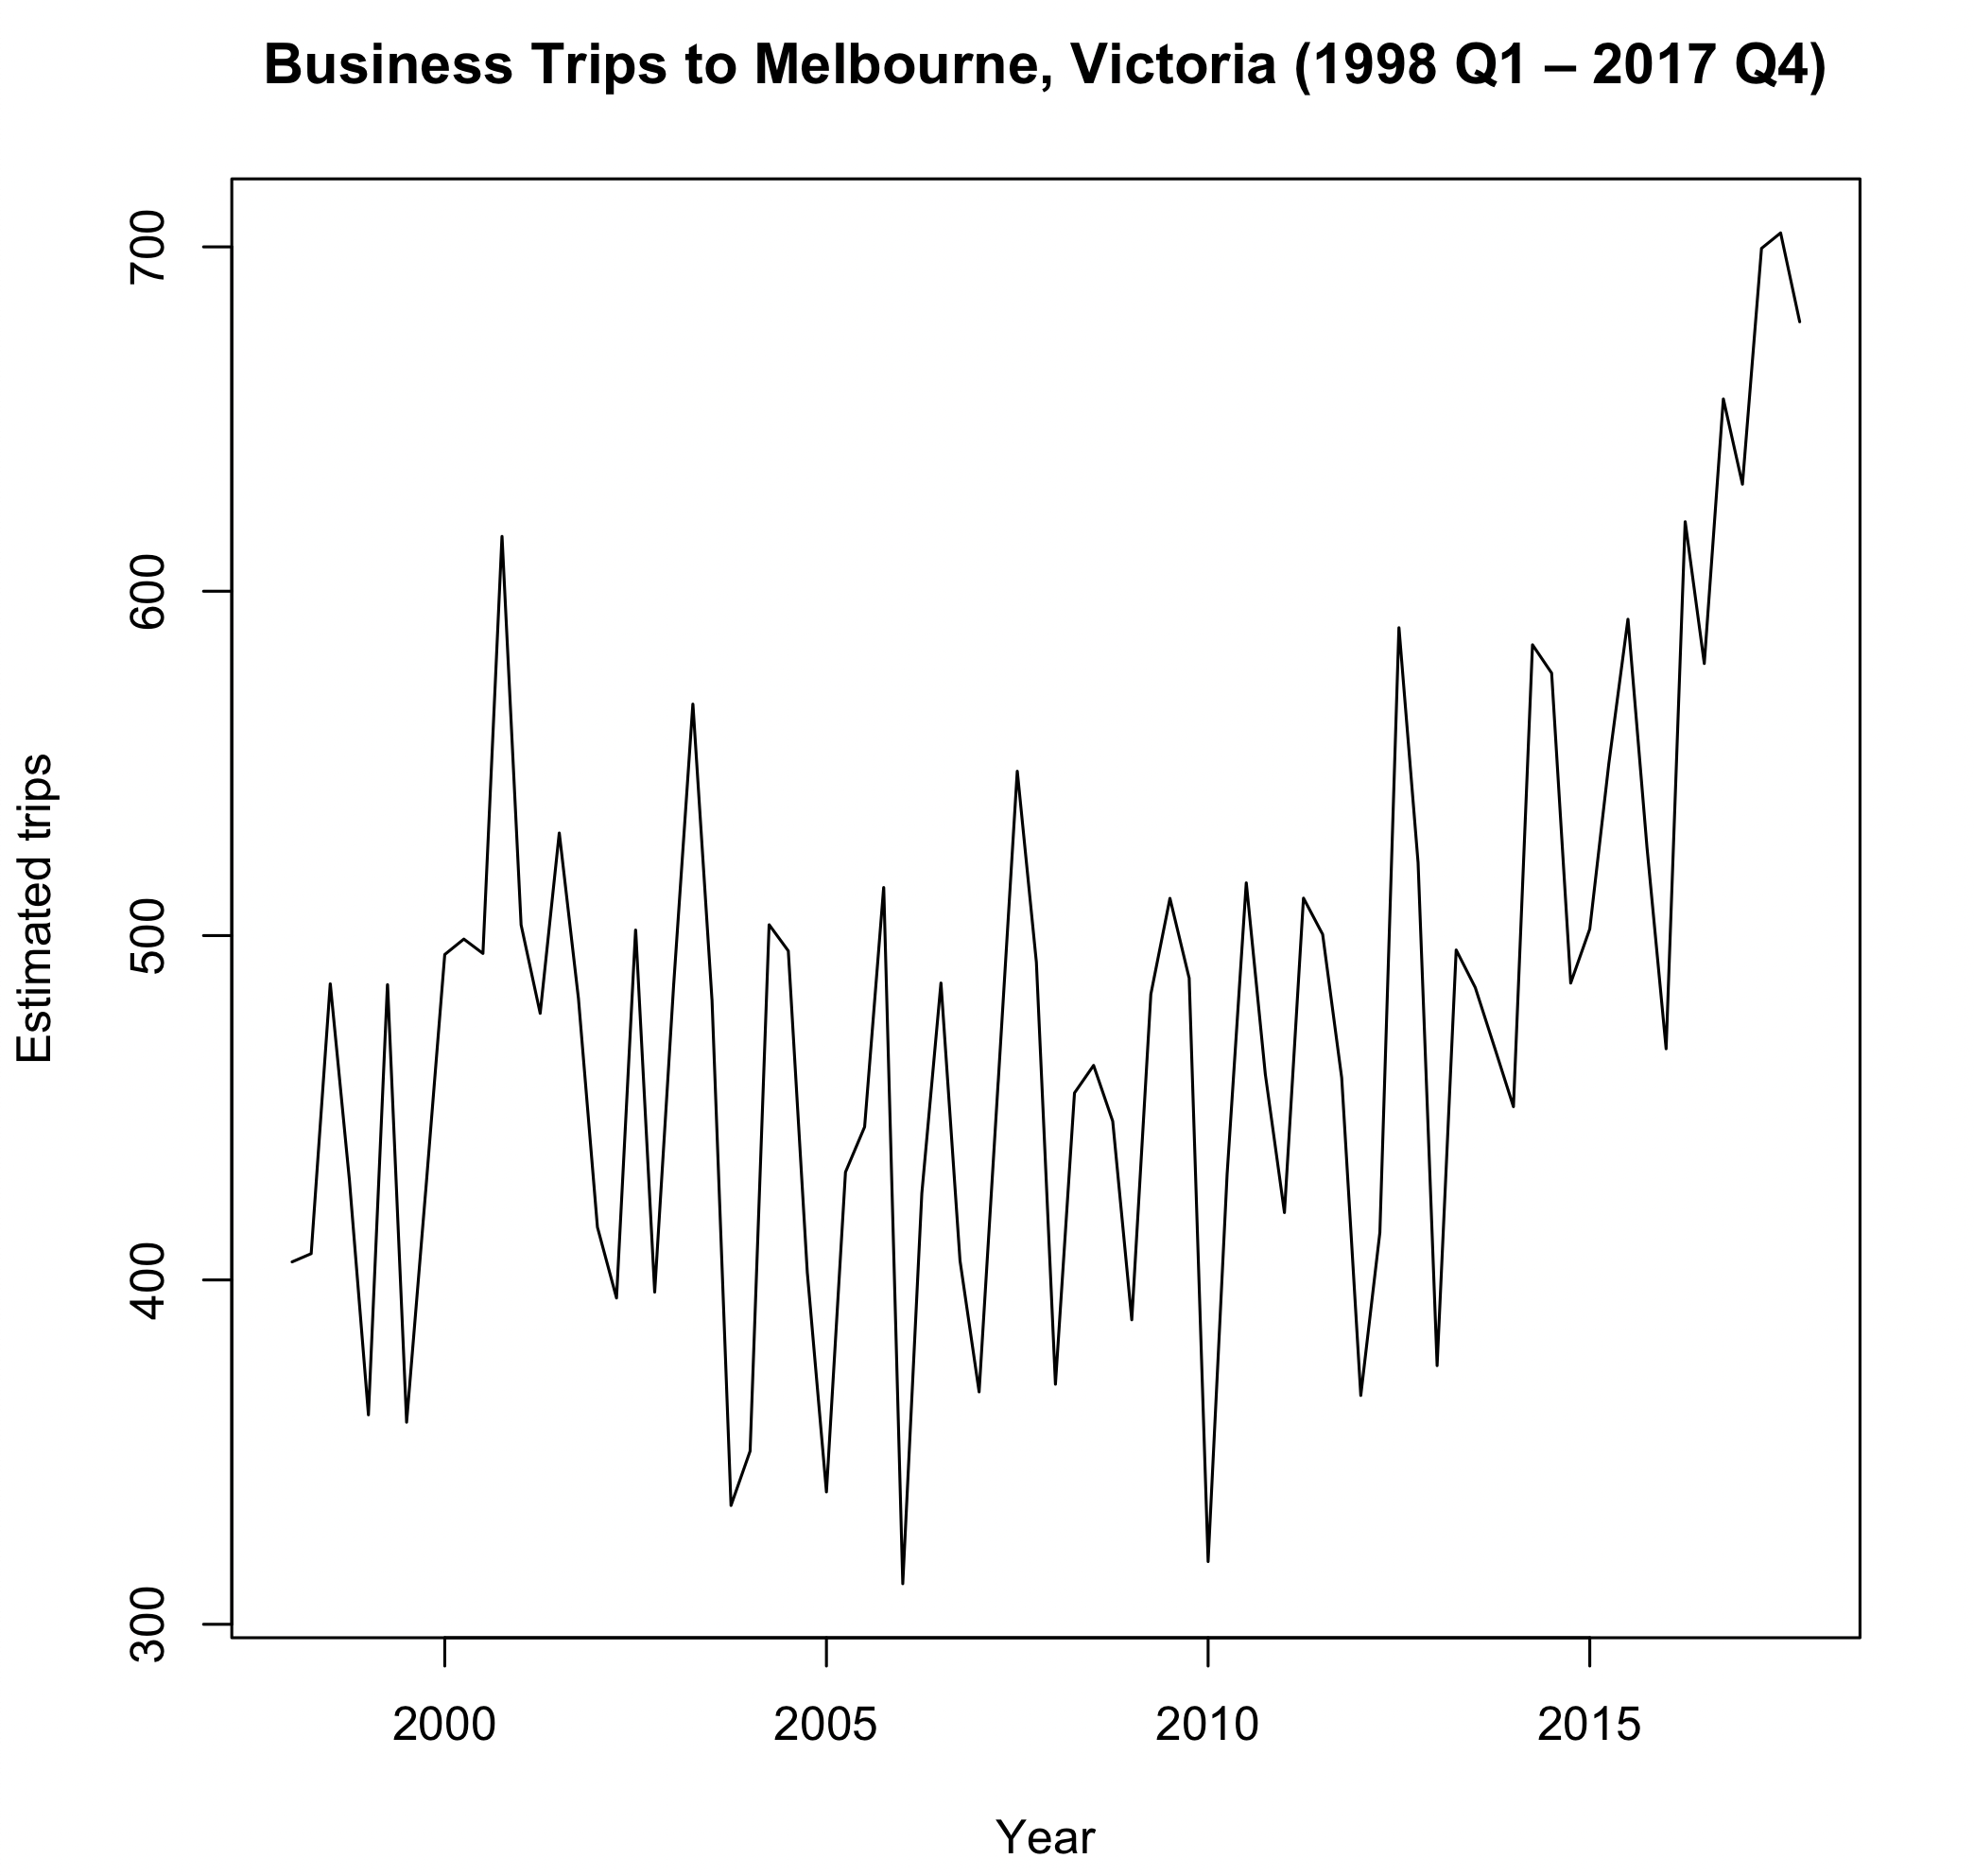
\includegraphics[width=0.55\linewidth]{fig/y1timeplot.png}
\end{figure}

\noindent The time plot exhibits two distinct phases. From 1998 to around 2010, the series fluctuates without a clear trend. From 2010 onwards, it shows a strong upward trend, accelerating after 2014 and reaching a peak of approximately 700 trips in 2017. A clear annual seasonal pattern is also evident throughout the period. Overall, the average number of Business trips increased from about 400 in 1998 to 700 in 2017, representing an increase of approximately 57\%.
% \begin{lstlisting}[language=R]
% layout(1:2)
% plot(aggregate(y1))
% \end{lstlisting}

\begin{figure}[H]
    \centering
    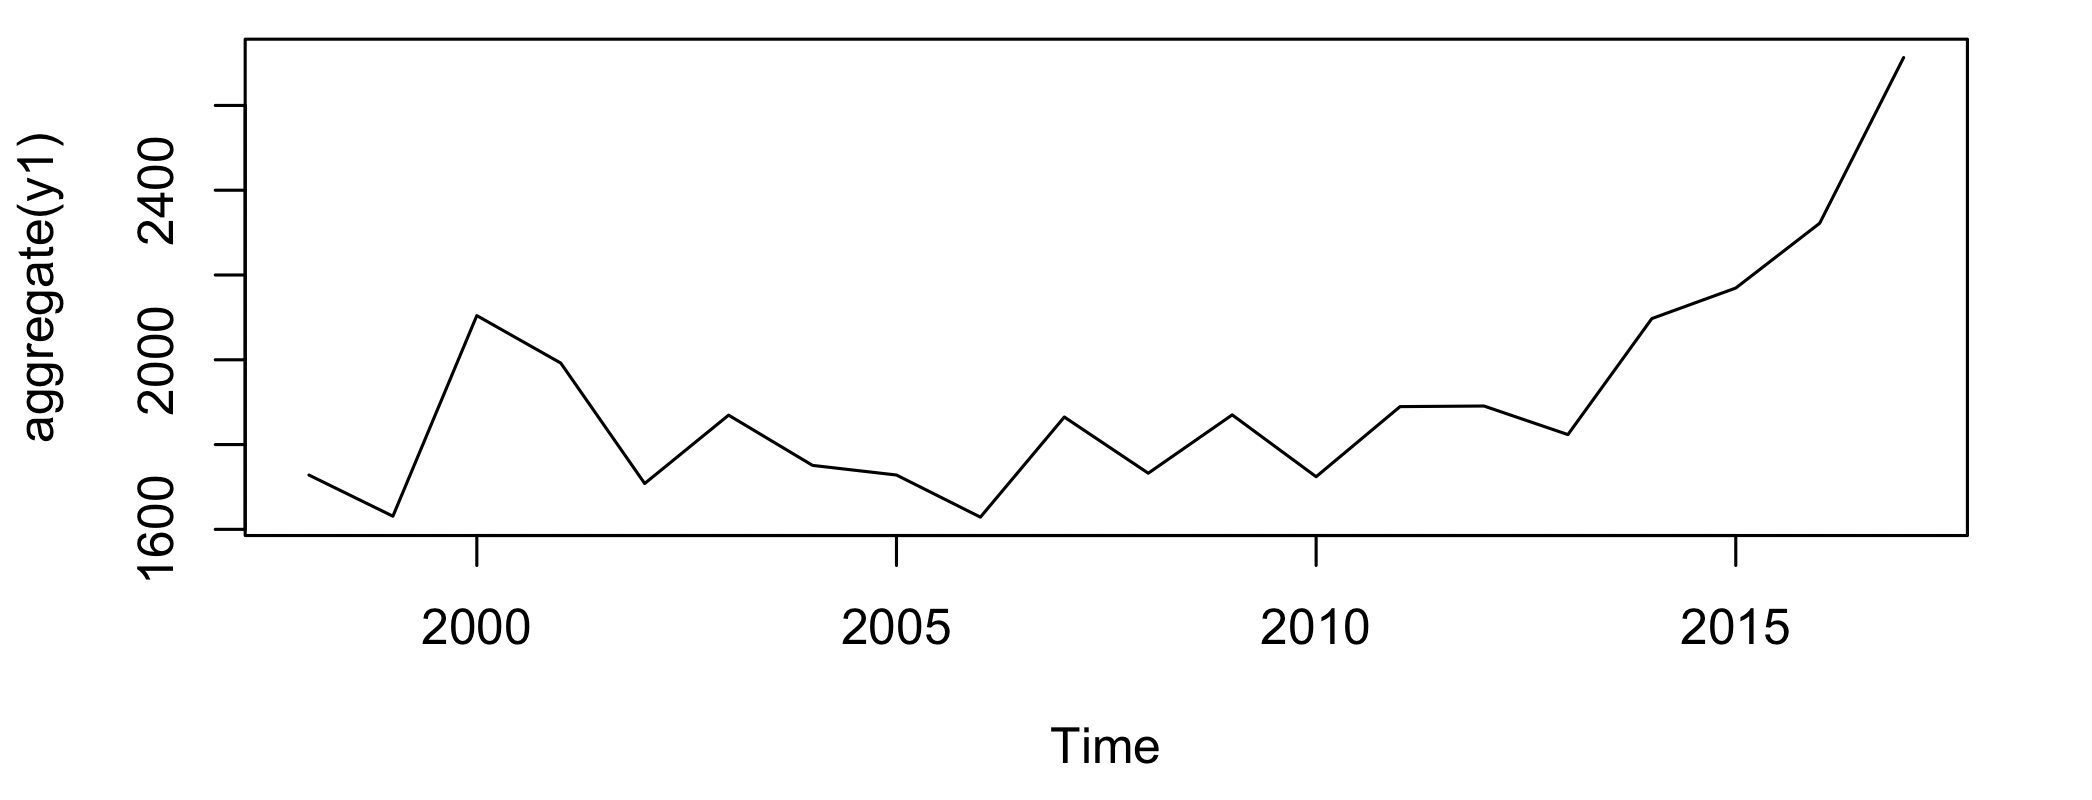
\includegraphics[width=0.65\linewidth]{fig/y1aggregate.png}
\end{figure}
\noindent To get a clearer view of the trend, the seasonal effect can be removed by aggregating the data to annual level.
\noindent It is apparent from the annual series that the number of business trips to Melbourne is increasing over time. The annual total is approximately 1728 trips in 1998, reaching a total of approximately 2713 trips by 2017. Aligned with our previous observations, the plot does not show any clear directional movement from around 2002 to 2010, and continues with a clear and continuous upward trend afterwards.
\pagebreak
\noindent Additionally, with the boxplot of the series, we can further see the seasonal effects.\\

% \begin{lstlisting}[language=R]
% boxplot(y1 ~ cycle(y1),
% 		names = c("Q1","Q2","Q3","Q4"),
% 		main = "Seasonal boxplot of Business Trips",
% 		xlab = "Quarter", ylab = "Number of Trips")
% \end{lstlisting}

\begin{figure}[H]
    \centering
    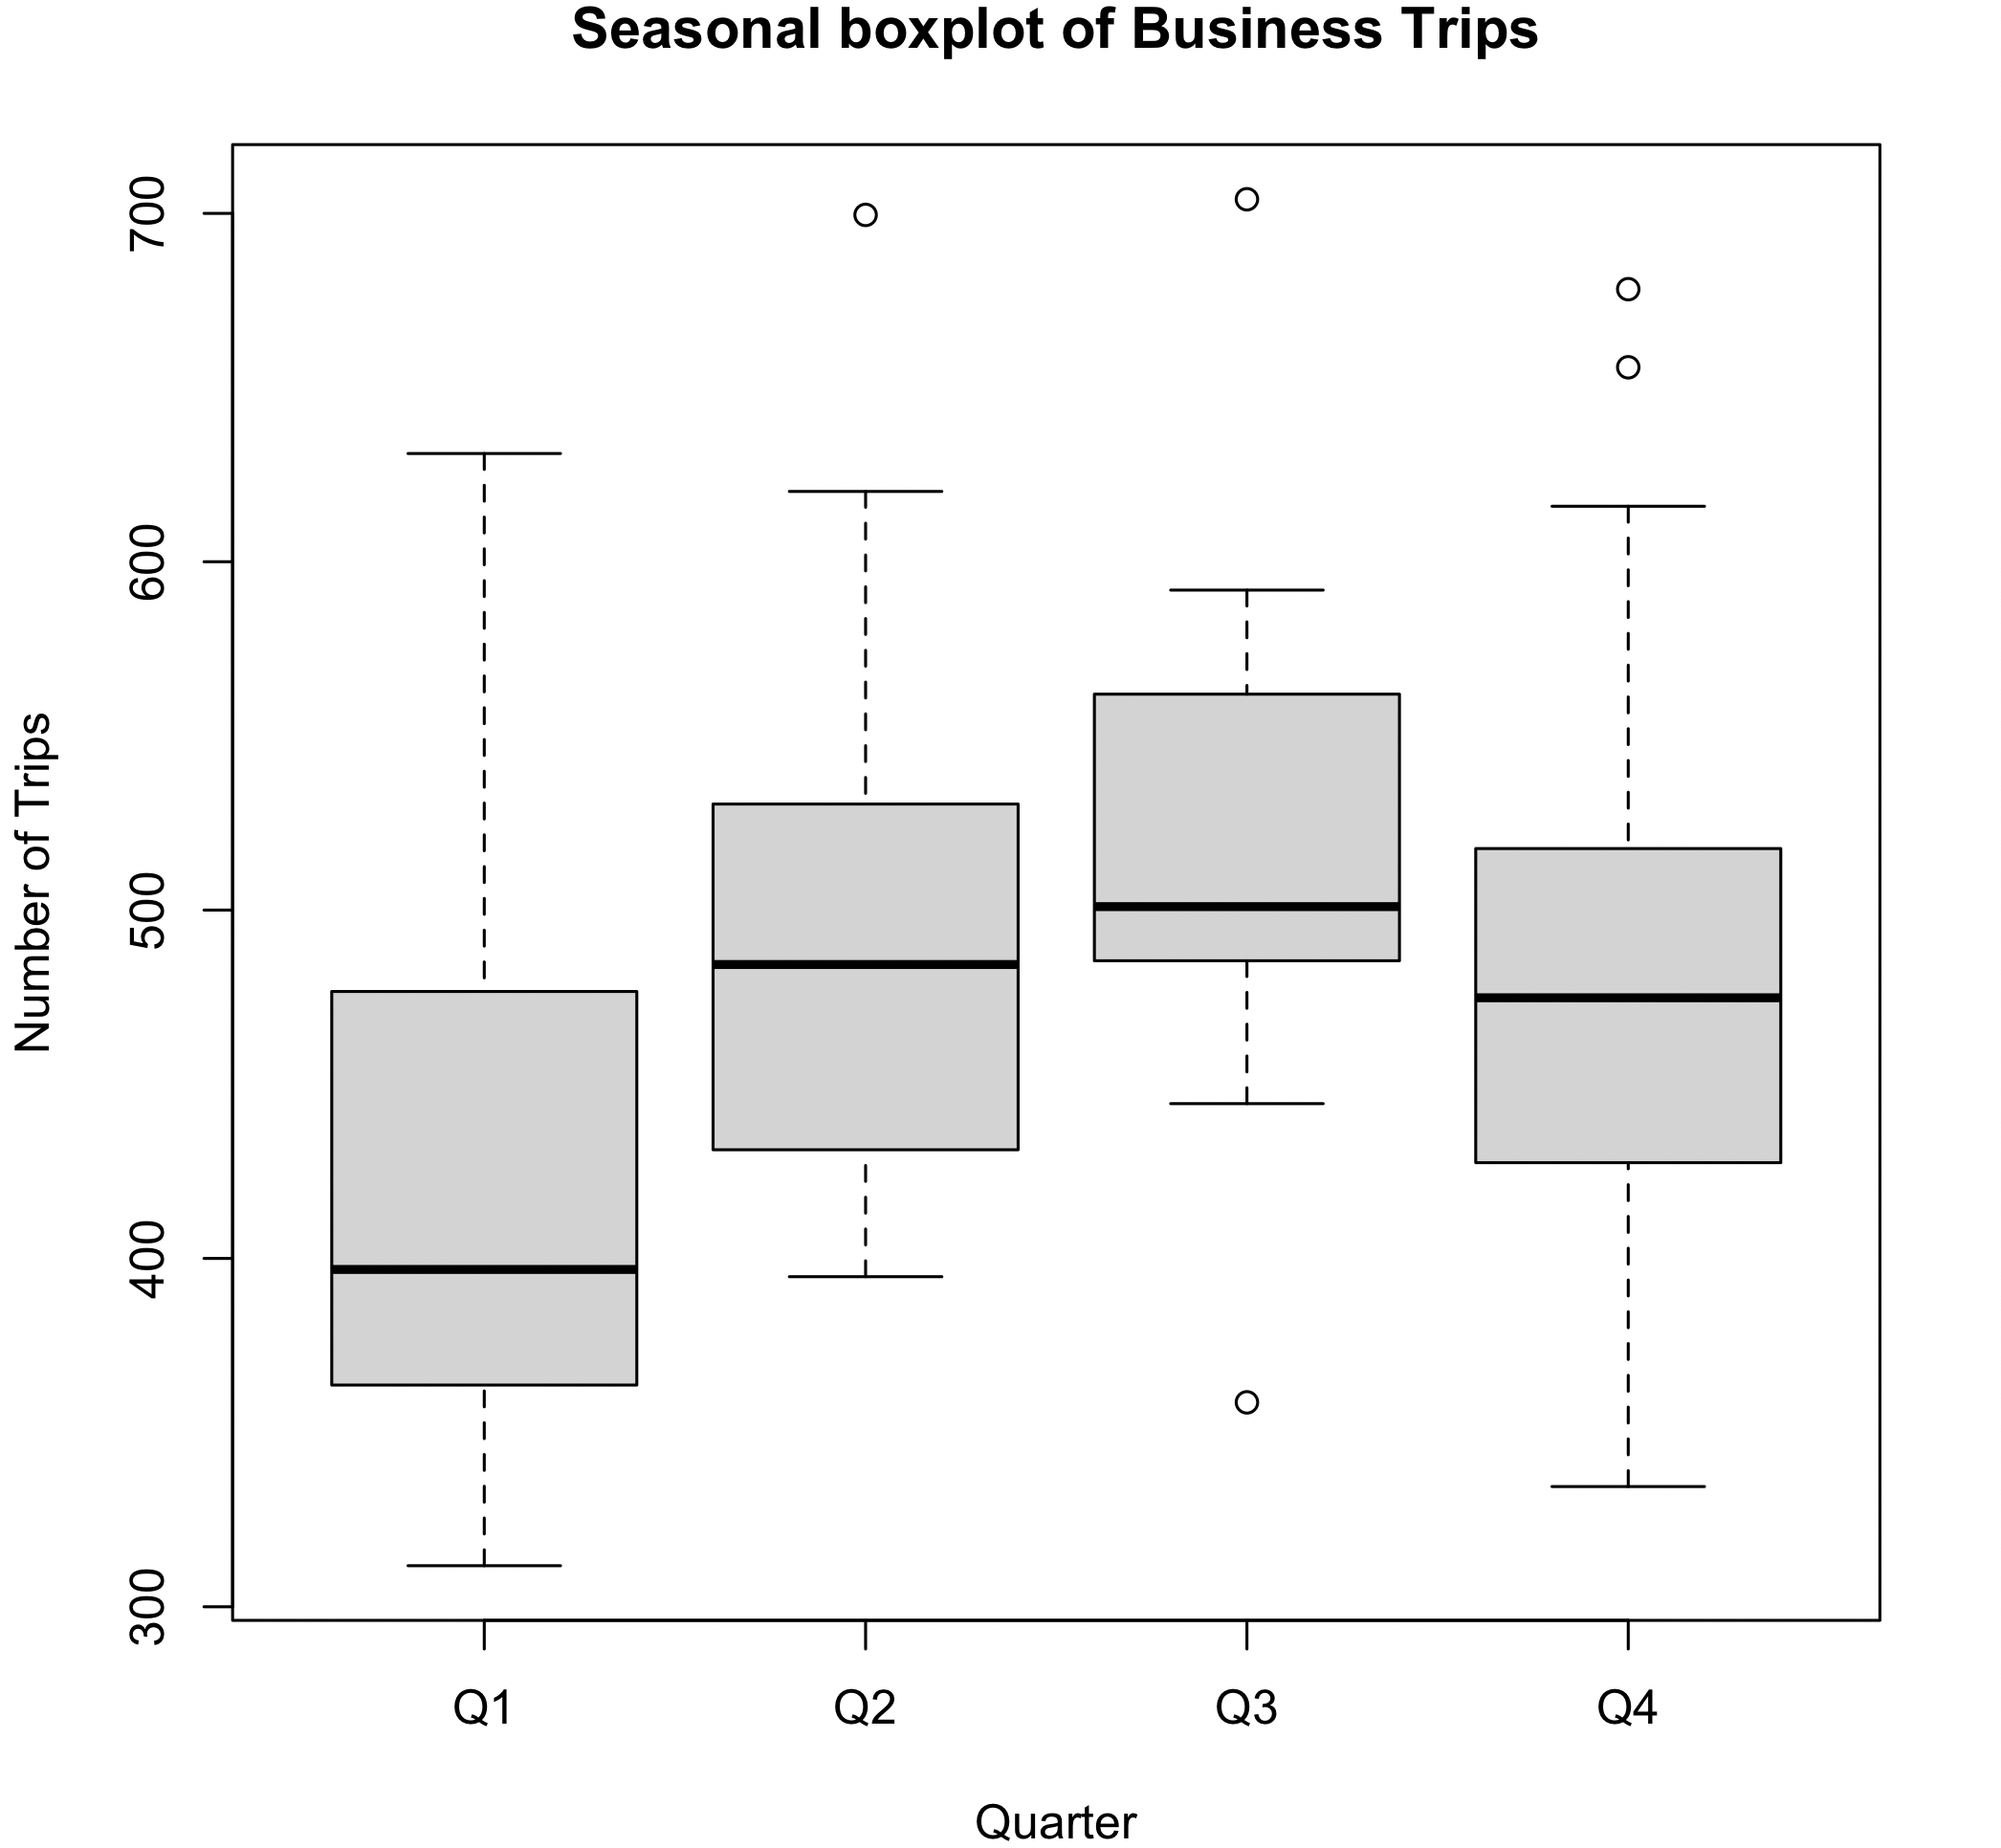
\includegraphics[width=0.55\linewidth]{fig/y1boxplot.png}
\end{figure}

\noindent Trip bookings are highest during July to September with an average of approximately 500 trips, and lowest during January to March with an average of approximately 400 trips. Q2 and Q4 falls in between, averaging approximately 490 trips. The differences across quarters are apparent, confirming that business travels to Melbourne is strongly dependent on the time of year.\\
\noindent A possible explanation for this seasonal pattern, is that business activities tend to be higher in the middle of the year.

\subsection{Holiday Series}
\begin{figure}[h]
    \centering
    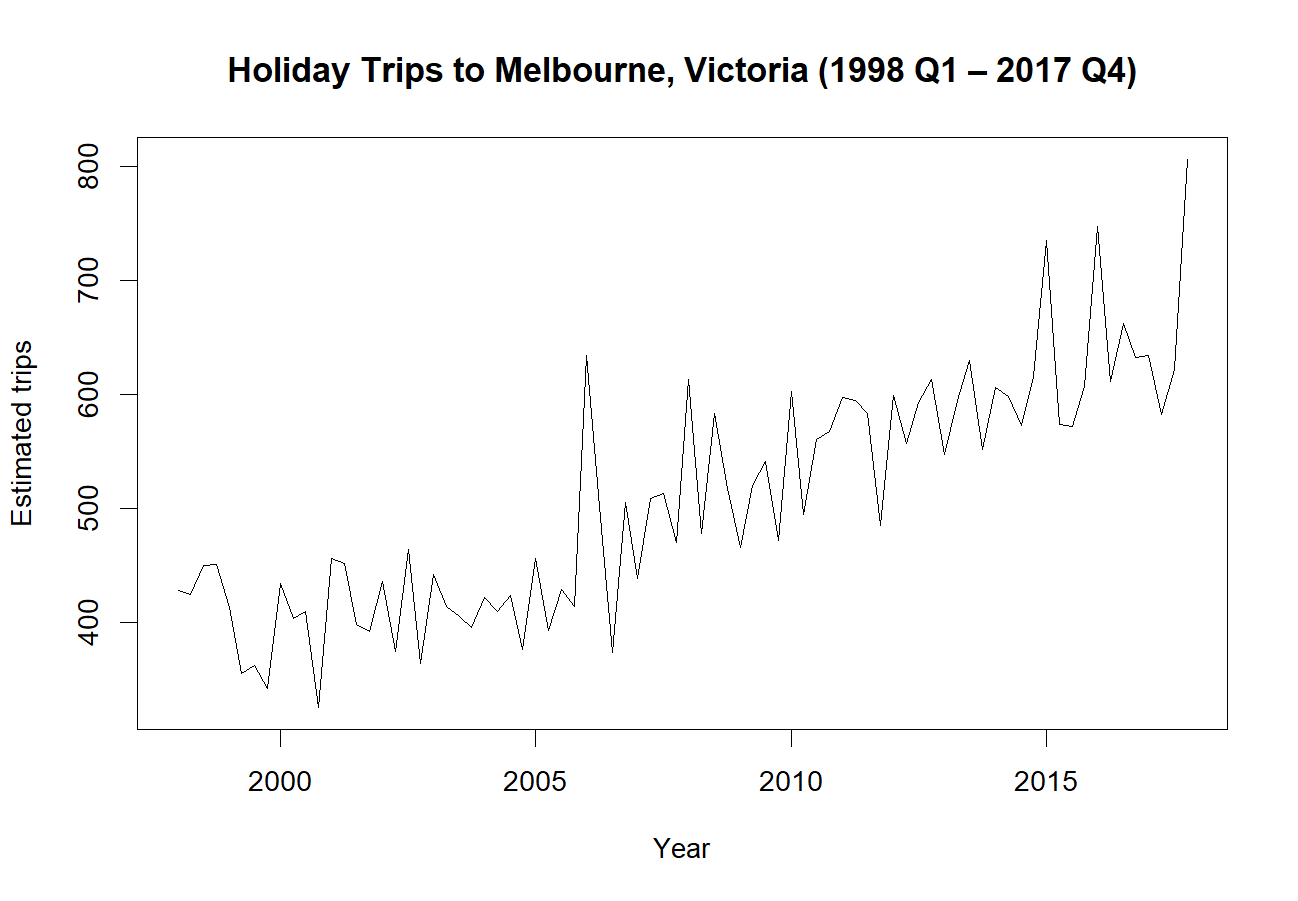
\includegraphics[width=0.55\linewidth]{fig/figy2timeplot.png}
\end{figure}

\noindent The time plot shows that different phases over the observation period. From 1998 to around 2005, the series fluctuates around a relatively stable level without a clear trend. From 2006 onwards, it shows an upward trend, which becomes more pronounced after 2010, reaching a peak of approximately 800 trips in 2017. A clear annual seasonal pattern is also evident throughout the period. Overall, the average number of Holiday trips increased from about 400 in 1998 to 800 in 2017, representing an increase of approximately 100\%.

\begin{figure}[h]
    \centering
    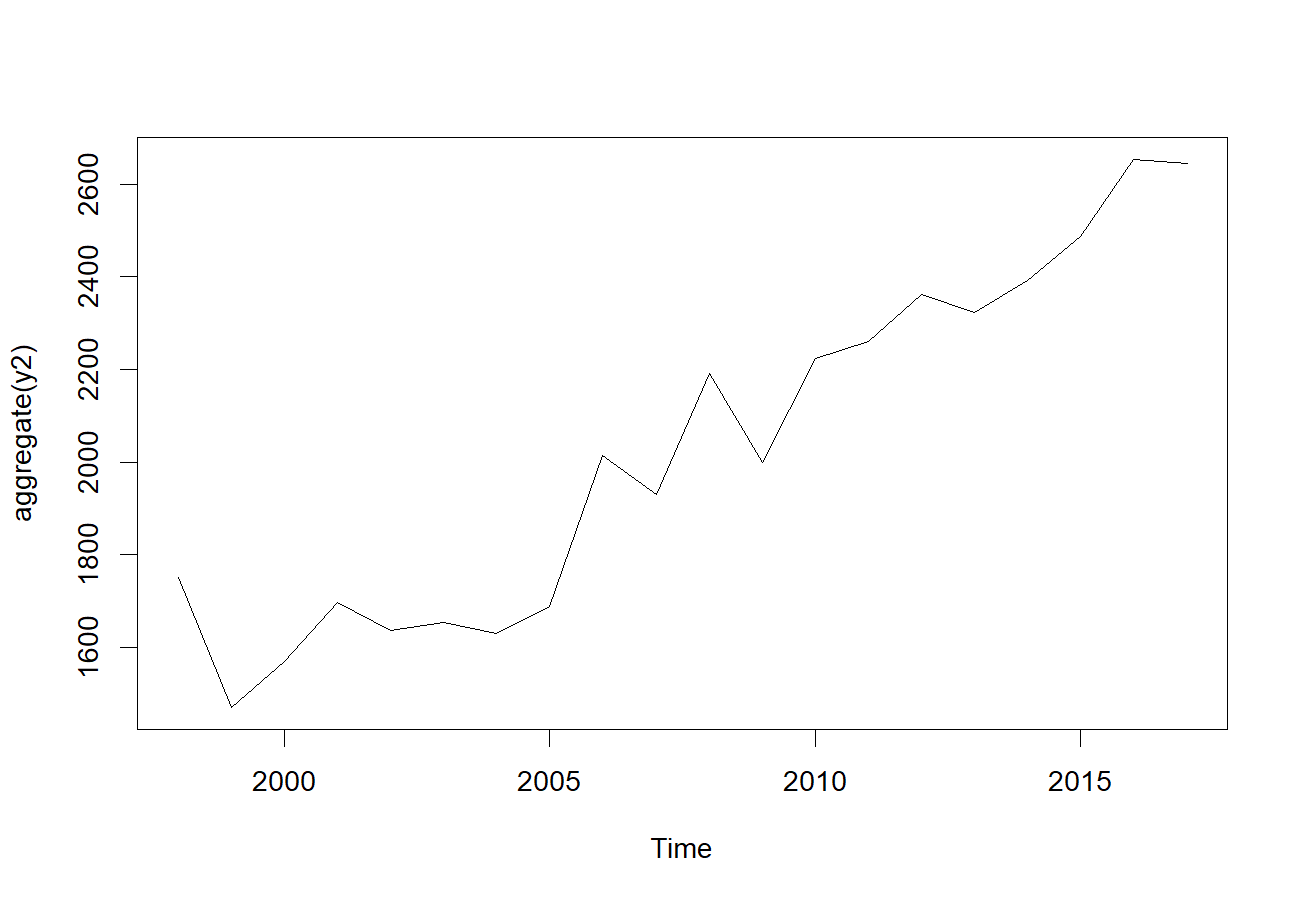
\includegraphics[width=0.65\linewidth]{fig/y2aggregate.png}
\end{figure}

\noindent To obtain a clearer view of the long-term trend, the seasonal effect can be reduced by aggregating the quarterly data into annual observations.
\noindent The aggregate plot confirms the overall increasing trend observed in the Holiday series. From 1998 to around 2005, the annual number of holiday trips remains relatively stable, fluctuating between approximately 1,500 and 1,700 trips. From 2006 onwards, the series exhibits a clear upward trend, although there are slight year-to-year fluctuations. The annual number of holiday trips increases steadily and reaches approximately 2,650 trips towards the end of the observation period, indicating sustained growth in holiday travel to Melbourne.
\noindent Thus, the quarterly boxplot of the series provides further evidence of seasonal variation.
\begin{figure}[h]
    \centering    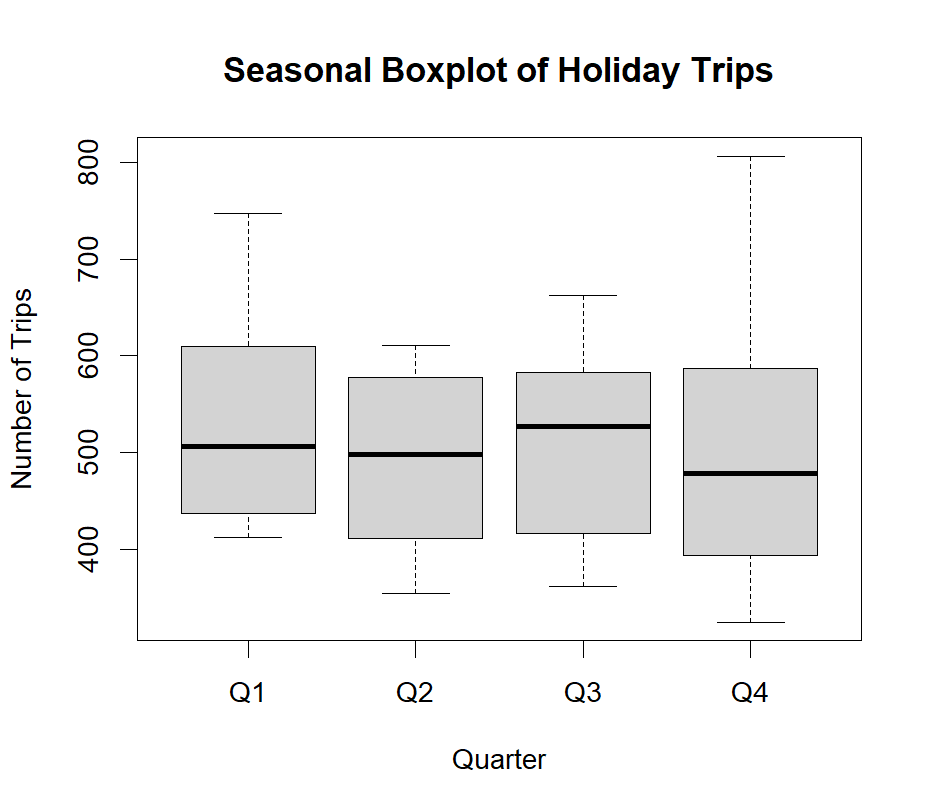
\includegraphics[width=0.55\linewidth]{fig/y2boxplot.png}
\end{figure}

\noindent The seasonal boxplot shows that the number of holiday trips varies across the four quarters. Quarter 3 has the highest median, at around 525 trips, while Quarter 4 has the lowest median, at around 480 trips. Quarter 1 and Quarter 2 fall in between, with median values of about 505 and 500 trips. Quarter 4 also shows a wider spread than the other quarters, meaning that the number of holiday trips is more variable during this quarter. Although the differences are not very large, they still suggest that holiday trips follow a seasonal pattern.\\
\noindent A possible explanation for this seasonal pattern is that holiday travel demand changes throughout the year due to factors such as school holidays and public holidays.

\subsection{Conclusion of the Two Series}

\noindent In conclusion, both Business and Holiday series show an increasing trend and clear quarterly seasonal patterns over the observation period. The Holiday series demonstrates a stronger growth trend compared to the Business series, while both series exhibit variations across different quarters. Therefore, trend and seasonal components should be considered when fitting appropriate time series models.
